\section{Case Study Evaluation}

% ============================================================
% S14: CASE STUDY 1 - FACIAL RECOGNITION
% ============================================================
\begin{frame}{Case Study 1: Metropolitan Police Live Facial Recognition}
    \begin{columns}[T]
        \begin{column}{0.48\textwidth}
            \textbf{Baseline Scores:} Fairness 1.5, Privacy 1.5, Safety 5.0 (1--7 Likert scale).

            \vspace{6pt}
            \textbf{Results (All Frameworks):}
            \begin{itemize}
                \item Overall: \textbf{0.3866} (Critical).
                \item Developer: 0.4826.
                \item Affected Community: 0.3063.
            \end{itemize}

            \vspace{6pt}
            \textbf{Conflict:} Low (all $\rho > 0.89$). The extreme ethical profile creates clear ranking agreement.
        \end{column}
        \begin{column}{0.48\textwidth}
            \centering
            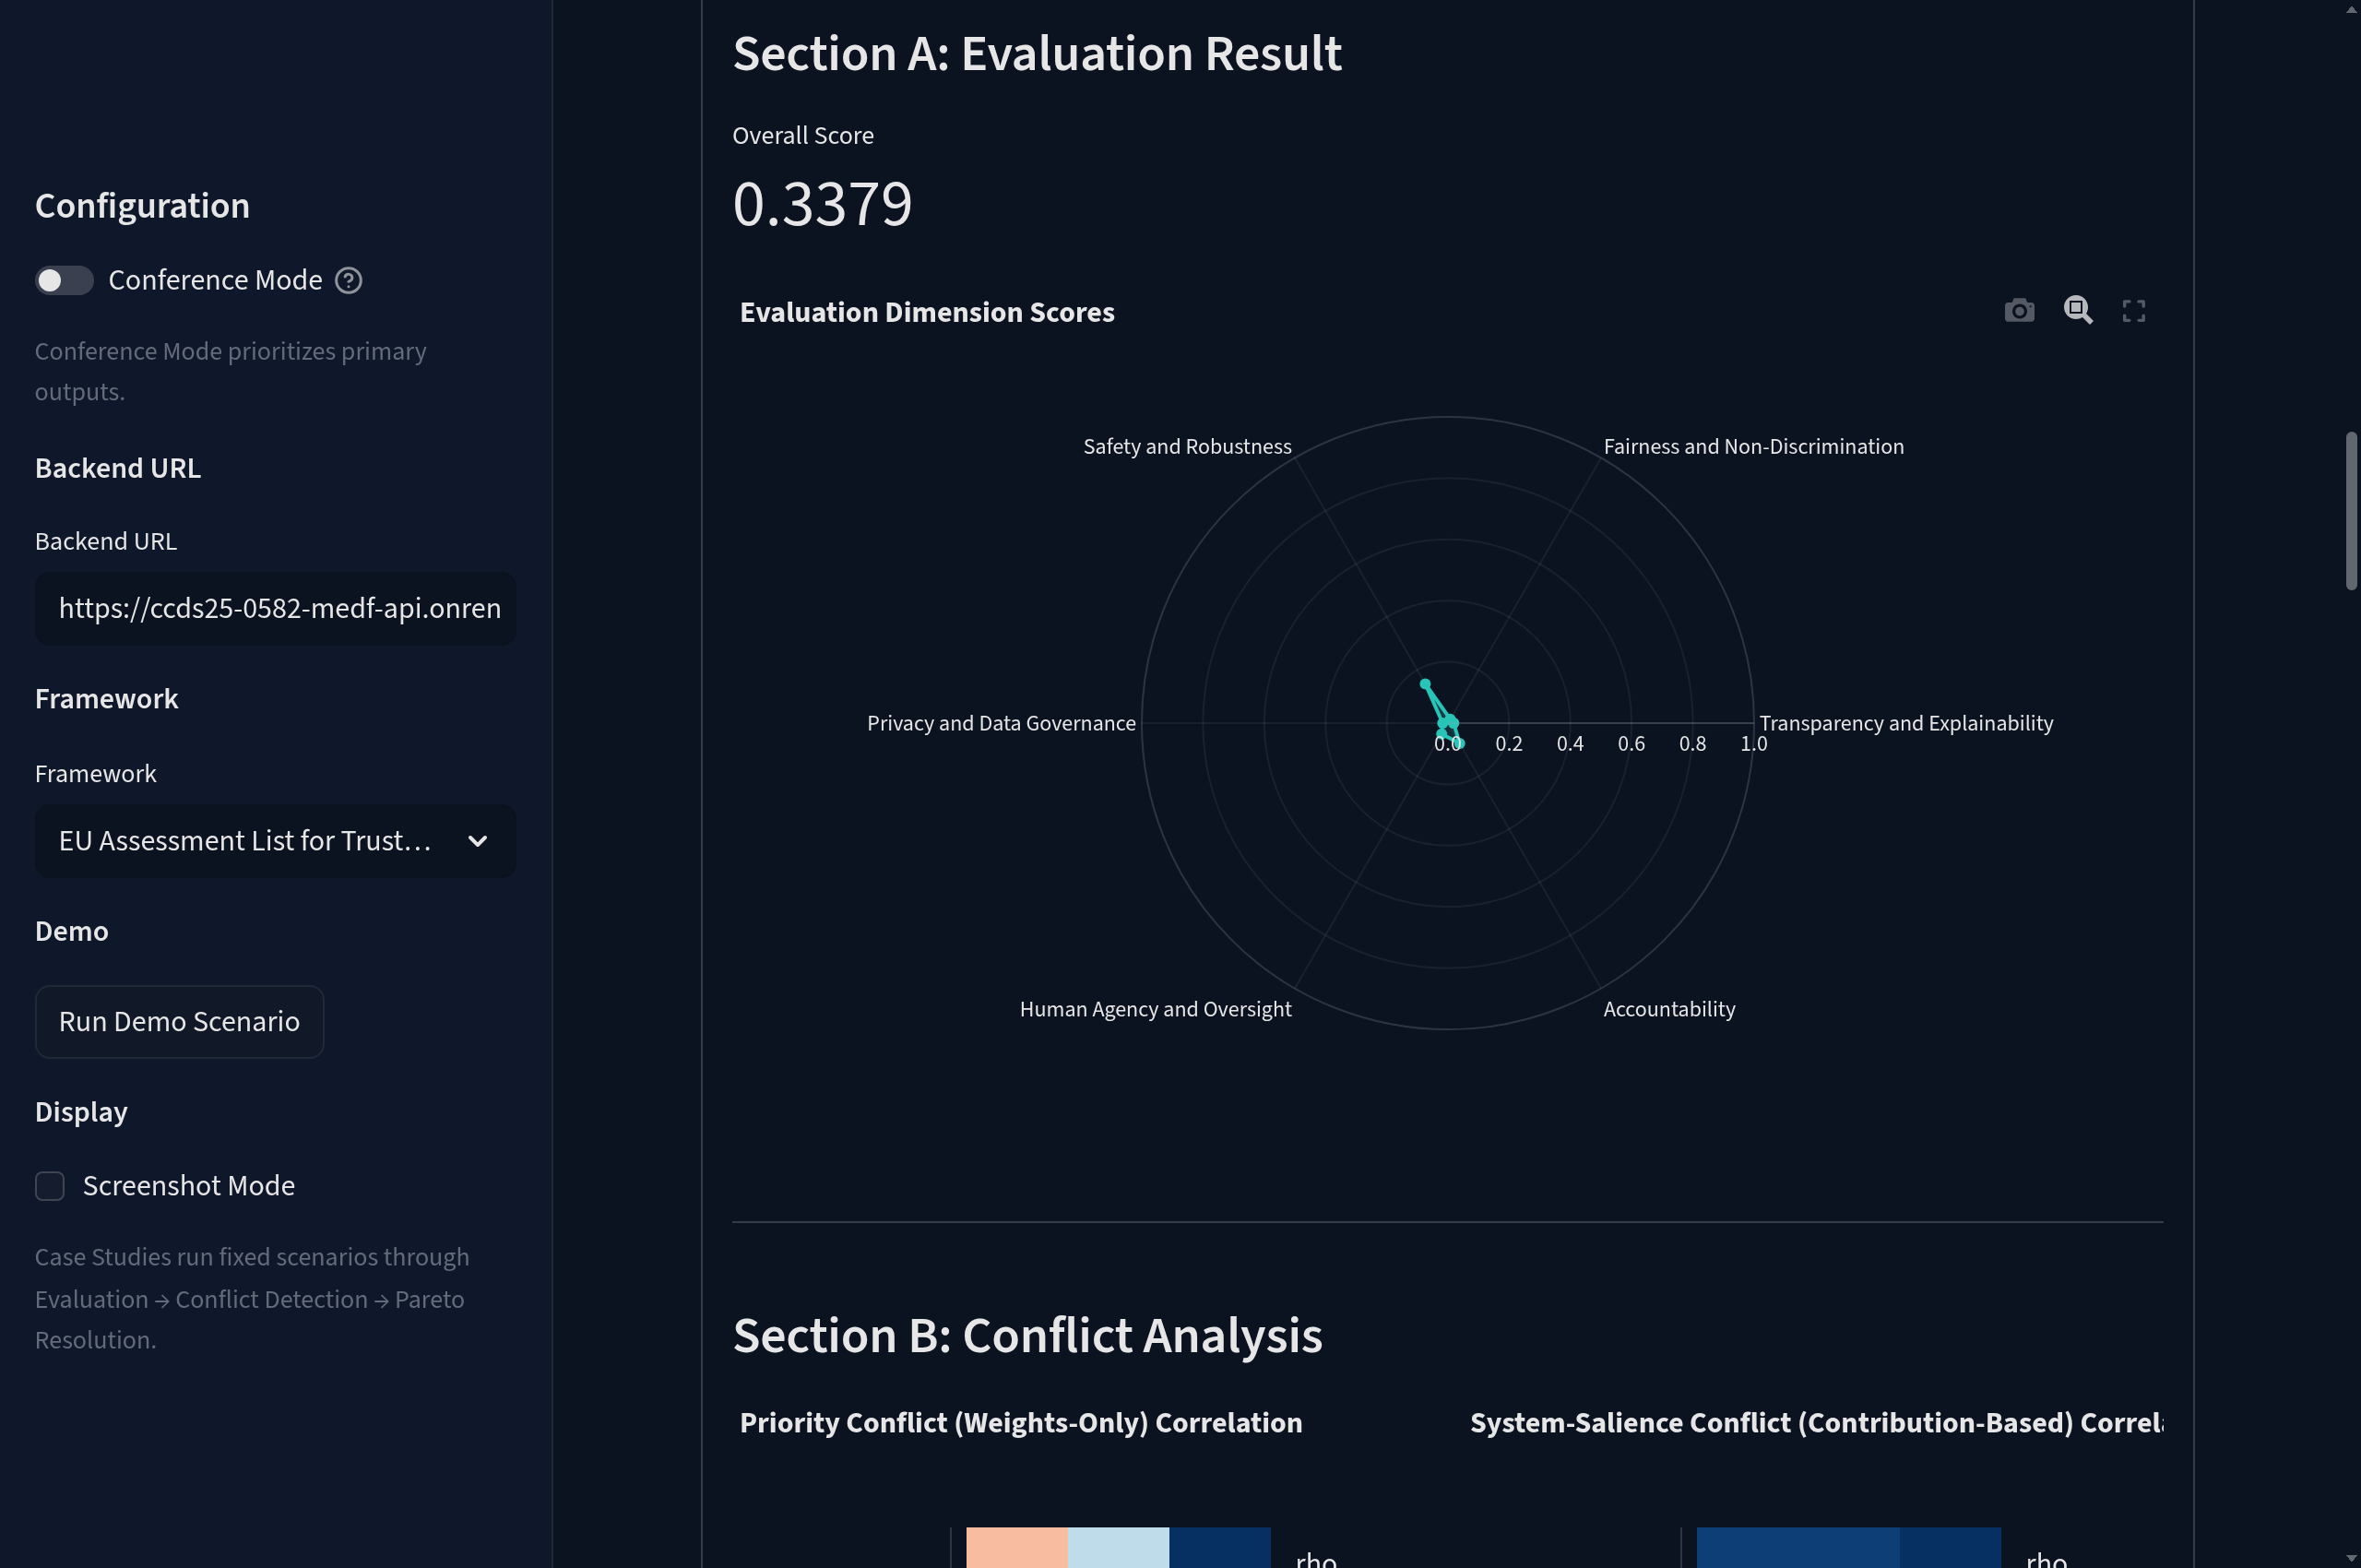
\includegraphics[width=\linewidth,height=0.55\textheight,keepaspectratio]{images/fig_10_6_casestudy1.png}

            {\footnotesize Figure 10.6: Case Study 1 evaluation results (overall score 0.3379).}
        \end{column}
    \end{columns}
\end{frame}
% NOTES: The facial recognition case has severe failures on Fairness and Privacy.
% Despite different absolute scores, all stakeholders agree on the dimension ranking.
% Approximately 60 seconds.
% Transition: "The hiring algorithm case shows a different conflict pattern."

% ============================================================
% S15: CASE STUDY 2 - HIRING ALGORITHM
% ============================================================
\begin{frame}{Case Study 2: iTutorGroup Automated Hiring}
    \textbf{System Description:} Automated rejection of applicants over age 55~\cite{eeoc2022itutorgroup}. Deliberate, systemic age discrimination.

    \vspace{8pt}
    \textbf{MEDF Evaluation Results (All Frameworks):}
    \begin{itemize}
        \item Overall: \textbf{0.3477} (Critical risk). A single catastrophic ethical flaw renders the system unacceptable from every stakeholder perspective.
        \item Conflict: Moderate ($\rho = 0.54$ Developer-Regulator). The ambiguous ethical profile exposes genuine disagreement.
        \item The Regulator scores higher (0.4004) due to Accountability emphasis, while the Affected Community scores lowest (0.3005).
    \end{itemize}
\end{frame}
% NOTES: This case demonstrates MEDF's ability to correctly penalize systems with
% catastrophic single-dimension failures. Approximately 60 seconds.
% Transition: "The NHS-DeepMind case reveals the highest stakeholder conflict."

% ============================================================
% S16: CASE STUDY 3 - NHS-DEEPMIND
% ============================================================
\begin{frame}{Case Study 3: Royal Free NHS-DeepMind Streams}
    \textbf{System Description:} Clinical AKI detection app. Life-saving benefit, but 1.6M patient records accessed without consent~\cite{ico2017deepmind}.

    \vspace{8pt}
    \textbf{MEDF Evaluation Results (All Frameworks):}
    \begin{itemize}
        \item Overall: \textbf{0.6003} (Medium risk). The genuine clinical benefit (Safety 6.0) partially offsets the Privacy failure (3.5).
        \item Conflict: High ($\rho = -0.14$ Developer-Regulator). The balanced ethical profile exposes real stakeholder tension.
        \item This is the most genuinely contentious case: the Developer values clinical utility while the Regulator prioritizes data governance.
    \end{itemize}
\end{frame}
% NOTES: This case demonstrates the full power of the contribution-based conflict metric.
% Unlike the facial recognition case, the balanced profile here exposes genuine disagreement.
% Approximately 60 seconds.
% Transition: "Comparing all three cases reveals the critical finding of this project."

% ============================================================
% S17: CROSS-CASE COMPARISON
% ============================================================
\begin{frame}{Cross-Case Comparative Analysis}
    \centering
    \setlength{\tabcolsep}{4pt}
    \begin{tabular}{l c c c c}
        \toprule
        \textbf{Case Study} & \textbf{Overall} & \textbf{Risk} & \textbf{Min $\rho$} & \textbf{Conflict} \\
        \midrule
        Facial Recognition   & 0.3866 & Critical & 0.89  & Low \\
        iTutorGroup Hiring   & 0.3477 & Critical & 0.54  & Moderate \\
        NHS-DeepMind Streams & 0.6003 & Medium   & $-0.14$ & High \\
        \bottomrule
    \end{tabular}

    \vspace{8pt}
    {\small \textbf{Critical Finding:} Contribution-based conflict analysis differentiates genuinely contentious cases from clear ethical violations, even when using identical default stakeholder weights.}
\end{frame}
% NOTES: This table is the summary artifact for the case study evaluation. The inverse
% relationship between ethical severity and conflict level is the central insight.
% Approximately 60 seconds.
% Transition: "Let me now address the limitations of this work."
